\documentclass[a4paper]{article}
\usepackage[utf8x]{inputenc}
\usepackage[english]{babel}

\usepackage[margin=2cm]{geometry}
\usepackage{amsmath}

\pagestyle{empty}



\usepackage{tikz}
\usetikzlibrary{calc}


\begin{document}
\setlength\unitlength{3cm}
\subsection*{Notation}
	\begin{center}\begin{tikzpicture}[x=1\unitlength,y=1\unitlength]
		\node[opacity=0.2, draw=black, inner sep=0mm] (CAR) {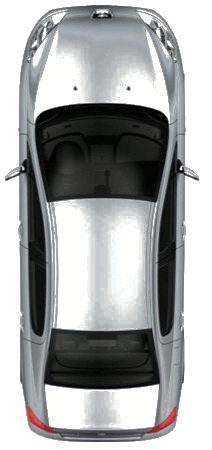
\includegraphics
					[width=1\unitlength,height=2\unitlength]{../car2.png}};

		\draw[thick, -to] ($(CAR.south) +(0,-2mm)$) -- ($(CAR.north) +(0,2mm)$);
		\draw[thick, -to] ($(CAR.west) + (-2mm,0)$) -- ($(CAR.east) + (2mm,0)$);

	\end{tikzpicture}\end{center}

\end{document}
